\documentclass{beamer}
\usefonttheme[onlymath]{serif}
% does not look nice, try deleting the line with the fontenc.
\usepackage[english]{babel}
\usepackage{amsmath}
\usepackage[latin1]{inputenc}
\usepackage{units}
\usepackage{colortbl}
\usepackage{multimedia}
\usepackage{bm}

\mode<presentation>
{
  \usetheme{Boadilla}
  \useoutertheme{infolines}
  \setbeamercovered{transparent} 
}

\newcommand{\Name}{\emph{dynoNet}}

\title[\Name]{\Name: a neural network architecture for learning dynamical systems}

%\subtitle{Industrial-scale experimental results\\} % (optional)

\author[]{Marco Forgione, Dario Piga}

\institute[IDSIA]{
	\inst{1}IDSIA Dalle Molle Institute for Artificial Intelligence SUPSI-USI, Lugano, Switzerland 
	} 


\date[]{\today}


\subject{System identification with neural networks}


%% MATH DEFINITIONS %%
\newcommand{\q}{q} % shift operator
\newcommand{\A}{A} % autoregressive polynomial
\newcommand{\ac}{a} % autoregressive polynomial coefficient
\newcommand{\B}{B} % exogenous polynomial
\newcommand{\bb}{b} % exogenous polynomial coefficient
\newcommand{\Gmat}{\mathbb{G}} % transfer function operator in matrix form
\newcommand{\tvec}[1]{\mathbf{#1}}
\newcommand{\mat}[1]{\bm{#1}}
\newcommand{\sens}[1]{\tilde{#1}}
\newcommand{\adjoint}[1]{\overline{#1}}
\newcommand{\loss}{\mathcal{L}}
\newcommand{\pdiff}[2]{\frac{\partial #1}{\partial #2}}
\newcommand{\nsamp}{T}

\newcommand{\conv}{*}
\newcommand{\ccorr}{\star}
%\newcommand{\R}{\mathcal{R}}
%\newcommand{\du}{\delta u}
%\newcommand{\dy}{\delta y}
%\newcommand{\DU}{\Delta U}
%\newcommand{\DY}{\Delta Y}
%\newcommand{\abs}[1]{\left | #1 \right |}
\newcommand{\norm}[1]{\left \lVert #1 \right \rVert}
%\newcommand{\relphantom}[1]{\mathrel{\phantom{#1}}}
%\newenvironment{matrixc}{\begin{array}{c}\left[}{\end{array}\right]}
\DeclareMathOperator*\argmin{arg \, min}
%\DeclareMathOperator*\argmax{arg \, max}
%\DeclareMathOperator*\fit{fit}
%\DeclareMathOperator*\RMSE{RMSE}
%\DeclareMathOperator*\diag{diag}
%\DeclareMathOperator*\diet{diet}
%\DeclareMathOperator*\Risk{Risk}
%\DeclareMathOperator*\Num{Num}
%\DeclareMathOperator*\Den{Den}
%\DeclareMathOperator*\Rat{Rat}
\DeclareMathOperator*\cov{cov}
%\DeclareMathOperator*\Var{Var}
%\DeclareMathOperator*\SSR{SSR}
%\setcounter{MaxMatrixCols}{20}
%\newcommand{\pdiff}[2]{\frac{\partial #1}{\partial #2}}
%\definecolor{mypink1}{rgb}{0.858, 0.188, 0.478}
%\definecolor{olive}{RGB}{85, 107, 47}
\definecolor{orange}{RGB}{204, 85, 0}

%\definecolor{mypink3}{cmyk}{0, 0.7808, 0.4429, 0.1412}
%\definecolor{mygray}{gray}{0.6}
%\definecolor{olivegreen}[RGB]{85, 107, 47}

\newcommand{\K}{K}
\newcommand{\M}{M}
\newcommand{\Mo}{M_o}
\newcommand{\So}{S_o}
\newcommand{\Smod}{S}
\newcommand{\parcolor}[1]{{\color{orange}#1}}
\newcommand{\Ts}{T_s^{\rm MPC}}
\newcommand{\cites}[1]{\begin{small}(#1)\end{small}}
%\newcommand{\Ts}{T_s}

\definecolor{darkgreen}{RGB}{20,150,50}
\definecolor{acq}{RGB}{119, 172, 48}
\definecolor{true}{RGB}{162, 20, 47}
\definecolor{surr}{RGB}{0, 114, 189}

\usepackage{listings}
% Default fixed font does not support bold face
\DeclareFixedFont{\ttb}{T1}{txtt}{bx}{n}{12} % for bold
\DeclareFixedFont{\ttm}{T1}{txtt}{m}{n}{12}  % for normal

\newcommand\pythonstyle{\lstset{
language=Python,
basicstyle=\ttb\tiny,
otherkeywords={self},             % Add keywords here
keywordstyle=\tiny\color{deepblue},
emph={MyClass,__init__},          % Custom highlighting
emphstyle=\ttb\color{deepred},    % Custom highlighting style
stringstyle=\color{deepgreen},
frame=tb,                         % Any extra options here
showstringspaces=false,            %
numberstyle=\footnotesize,
}}

\lstnewenvironment{python}[1][]
{
\pythonstyle
\lstset{#1}
}
{}

\begin{document}

\begin{frame}
  \titlepage
\end{frame}

\begin{frame}{Motivations}
Two main classes of \structure{neural network} structures for sequence modeling and system identification:
\begin{columns}
\column{.48\textwidth}
\begin{block}{Recurrent NNs}
 General state-space models
 \vskip 1em
    \begin{itemize}
     \item High representational capacity
     \item Hard to parallelize
     \item Numerical issues in training
    \end{itemize}
 \end{block}
\column{.48\textwidth}
\begin{block}{1D Convolutional NNs}
  Dynamics through FIR blocks
  \vskip 1em
    \begin{itemize}
     \item Lower capacity, several params
     \item Fully parallelizable
     \item Fast, well-behaved training
    \end{itemize}
\end{block}
\end{columns}

\pause
\vskip 2em
We introduce \Name\,: an architecture using linear {dynamical operators} parametrized as 
\structure{rational transfer functions} as  building blocks.
\pause
\vskip 1em
\begin{itemize}
\item Extends 1D Convolutional NNs to \structure{Infinite Impulse Response} dynamics
\item Can be trained efficiently by plain \structure{back-propagation}
\end{itemize}
\end{frame}


\begin{frame}{Related works}
\structure{Block-oriented} architectures consist in the interconnection of transfer functions $G(z)$ and static non-linearities $F(\cdot)$:
\begin{columns}
\column{.2\textwidth}
 \begin{figure}
 \footnotesize Wiener
 \vskip .5em
 \includegraphics[width=\textwidth]{img/wiener.pdf}
 \end{figure}
\column{.2\textwidth}
 \begin{figure}
 \footnotesize Hammerstein
 \vskip .5em
 \includegraphics[width=\textwidth]{img/hammer.pdf}
 \end{figure}
 \column{.3\textwidth}
 \begin{figure}
 \footnotesize Wiener-Hammerstein
 \vskip .5em
 \includegraphics[width=\textwidth]{img/wiener_hammerstein.pdf}
 \end{figure}
\end{columns}
\vskip 0em
%shallow architectures, SISO blocks \dots
\begin{columns}
\column{.4\textwidth}
 \begin{figure}
	 \footnotesize Generalized Hammerstein-Wiener
 \vskip .5em
 \includegraphics[width=\textwidth]{img/generalized_HW.pdf}
 \end{figure}
 \column{.4\textwidth}
 \begin{figure}
 \vskip 1em
 \footnotesize Parallel Wiener-Hammerstein
 \vskip 1em
 \includegraphics[width=.9\textwidth]{img/parallel_WH.pdf}
 \end{figure}
\end{columns}
\vskip 1em
extensively studied in System Identification.\\
\pause
Training with \structure{specialized algorithms} requiring, e.g. {analytic} expressions of gradients/jacobians.
%They are extensively studied in the system identification literature.

%\vskip 2em
%\pause

%\vskip 1em
%$G(z)$: transfer function. $F(\cdot)$: static non-linearity.
 \end{frame}

\begin{frame}{\Name}
\begin{itemize}
 \item  \Name\ generalizes block-oriented models to \structure{arbitrary connection} of MIMO blocks $G(z)$ and $F(\cdot)$
 \item More importantly, training is performed using a \structure{general approach} 
 \item Plain \structure{back-propagation} for gradient computation exploiting Deep Learning software
\end{itemize}
\begin{figure}
 \vskip 0em
 \footnotesize a \Name\ network
 \vskip .5em
 \includegraphics[width=.60\textwidth]{img/generic_layer.pdf}
\end{figure}
\pause
\alert{Technical challenge}: back-propagation through the transfer function! \\
No hint in the literature, no ready-made implementation available.
\end{frame}

\begin{frame}{Transfer function (SISO)}

Transforms an input sequence $u(t)$ to an output $y(t)$ according to:
\begin{footnotesize}
	$$y(t) = G(\q)u(t) = \frac{\bb_0 + \bb_1 \q^{-1} + \dots + \bb_{n_{\bb}}q^{-n_{\bb}}}{1 + \ac_1 \q^{-1} + \dots + \ac_{n_\ac}q^{-n_\ac}} u(t)$$
\end{footnotesize}
Equivalent to the recurrence equation:
\begin{footnotesize}
$$ y(t) = \bb_0 u(t) + \bb_1 u(t-1) + \dots + \bb_{n_\bb}\!u(t-n_\bb)-\ac_1 y(t\!-\!1) \dots - \ac_{n_\ac} y(t\!-\!n_\ac).$$
\end{footnotesize}
%\end{equation}

\pause

For our purposes, $G$ is a \structure{vector operator} with coefficients $a$, $b$, transforming $\tvec{u} \in \mathbb{R}^\nsamp$ to $\tvec{y} \in \mathbb{R}^\nsamp$
%\begin{footnotesize}
$$
 \tvec{y} = G(\tvec{u}; a, b)
$$
%\end{footnotesize}
\pause
%\vskip .5em
Our goal is to provide $G$ with a \structure{back-propagation} behavior.\\
The operation has to be \structure{efficient}!
\end{frame}

\begin{frame}{Forward pass}
In back-propagation-based training, the user defines a \structure{computational graph} producing a \structure{loss} $\loss$ (to be minimized). \\


\vskip 2em
In the \structure{forward pass}, the loss $\loss$ is computed.\\
$G$ receives $\tvec{u}$, $a$, and $b$ and needs to compute $\tvec{y}$:
\begin{columns}
\column{.5\textwidth}
$$
 \tvec{y} = G.\mathrm{forward}(\tvec{u}; a, b).
$$
\column{.5\textwidth}
\begin{figure}
\includegraphics[width=.8\textwidth]{img/forward_tf_ab.pdf}
\end{figure}
\end{columns}

\pause
\vskip 2em
The forward pass for $G$ is easy: it is just the filtering operation! \\
\vskip 1em
Computational cost: \color{darkgreen}{$\mathcal{O}(T)$}.
\end{frame}

 \begin{frame}{Backward pass}
 \begin{itemize}
 \item In the \structure{backward pass}, derivatives of $\loss$ w.r.t. the \structure{training variables} are computed. 
 Notation:  $\adjoint{x} = \pdiff{\loss}{x}$. 
 \item The procedure starts from $\adjoint{\loss} \equiv \pdiff{\loss}{\loss} = 1$ and goes \structure{backward}.
 \item Each operator must be able to ``push back'' derivatives from its outputs to its inputs
 \end{itemize}
 \vskip 1em

\uncover<2->{
 $G$ receives $\adjoint{\tvec{y}} \equiv \pdiff{\loss}{\tvec{y}}$ and is responsible for computing:
 $\adjoint{\tvec{u}}, \adjoint{a}, \adjoint{b}$:
 \begin{columns}
 \column{.5\textwidth}
 $$
  \adjoint{\tvec{u}}, \adjoint{a}, \adjoint{b} = G.\mathrm{backward}(\adjoint{\tvec{y}}; a, b).
 $$
 \column{.5\textwidth}
 \only<1>{
 \begin{figure}
 \includegraphics[width=.8\textwidth]{img/backprop_tf_ab_empty.pdf}
 \end{figure}
 }
 \only<2->{
 \begin{figure}
 \includegraphics[width=.8\textwidth]{img/backprop_tf_ab.pdf}
 \end{figure}
 }

 \end{columns}
}
 \vskip 1.5em
\uncover<3->{
%By defining these backward operations, we can use $G$ in Deep Learning!\\
%All \structure{technical details} are in the \Name\ arXiv paper\dots
 \structure{Chain rule} of calculus is the basic ingredient, but certain tricks may be used to \structure{speed up} the operation. Let us see an example...\\
}
 \end{frame}

 \begin{frame}{Backward pass for $\tvec{u}$}
 
 Compute $\adjoint{\tvec{u}} \equiv \pdiff{\loss}{\tvec{u}}$ from $\adjoint{\tvec{y}}\equiv \pdiff{\loss}{\tvec{y}}$. \\
 \pause
 \begin{itemize}
 \item Applying the chain rule:
 \begin{footnotesize}
$$\adjoint{\tvec{u}}_\tau = \pdiff{\loss}{\tvec{u}_\tau} 
= \sum_{t=0}^{\nsamp-1}{\pdiff{\loss}{\tvec{y}_t} \pdiff{\tvec{y}_t}{\tvec{u}_\tau}}
=\sum_{t=0}^{\nsamp-1}{\adjoint{\tvec{y}}_t \tvec{g}_{t-\tau}}
$$
\end{footnotesize}
where $\tvec{g}$ is the \structure{impulse response} of $G$.%contains the impulse response coefficients
\pause
\item From the expression above, by definition:
\begin{footnotesize}
$$\adjoint{\tvec{u}} = \tvec{g} \ccorr \adjoint{\tvec{y}},
$$
\end{footnotesize}
where  $\ccorr$ is \structure{cross-correlation}.
This implementation has cost  \alert{$\mathcal{O}(\nsamp^2)$}
\pause
\item It is equivalent to filtering $\adjoint{\tvec{y}}$ through $G$ in reverse time, and flipping the result. Implemented this way, the cost is {\color{darkgreen}{$\mathcal{O}(\nsamp)$}}! 
$$ \adjoint{\tvec{u}} = \mathrm{flip}\big(G(q) \mathrm{flip}(\adjoint{\tvec{y}})\big)$$
\pause  All details also for $\adjoint{a}$ and $\adjoint{b}$ in the \Name\ arXiv paper\dots
\end{itemize}
\end{frame}

\begin{frame}[fragile]{PyTorch implementation}
PyTorch implementation of the $G$-block in the repository \url{https://github.com/forgi86/dynonet}.
\vskip 1em
\centering
Use case:
\vskip 1em
\begin{columns}
 \column{.5\textwidth}
 \centering
 \Name \ architecture
\begin{figure}
 \vskip 0em
 \includegraphics[width=.8\textwidth]{img/generic_dynonet.pdf}
\end{figure}
 \column{.5\textwidth}
 \centering
 \vskip -.5em
 Python code
  \begin{tiny}
\begin{lstlisting}[language=python]


G1 = LinearMimo(1,  4, ...) # a SIMO tf
F = StaticNonLin(4, 3, ...) # a static NN
G2 = LinearMimo(3, 1, ...) # a MISO tf
G3 = LinearMimo(1, 1, ...) # a SISO tf
 
def model(in_data):  
    y1 = G1(in_data)
    z1 = F(y1) 
    y2 = G2(z1)
    out = y2 + G3(in_data)
    
\end{lstlisting}
\end{tiny}
\end{columns}
 \vskip 1em 
 \pause
 Any \structure{gradient-based} optimization algorithm can be used to train the \Name\ with derivatives  readily obtained by \structure{back-propagation}.
\end{frame}

\begin{frame}{Experimental results}
 Numerical experiments on public system identification benchmark available at \url{www.nonlinearbenchmark.org}.
 \begin{columns}
  \column{.33\textwidth}
   \centering
  \begin{figure}
  \footnotesize
  Wiener-Hammerstein\\
   \includegraphics[width=.99\textwidth]{img/WH_timetrace.pdf}
   $\mathrm{fit} = 99.5\%$
  \end{figure}
  \column{.33\textwidth}
  \begin{figure}
  \footnotesize
  Bouc-Wen
   \includegraphics[width=.99\textwidth]{img/BW_timetrace.pdf}
   $\mathrm{fit} = 93.2\%$
  \end{figure}
  \column{.33\textwidth}
  \begin{figure}
  \footnotesize
  EMPS
  \includegraphics[width=.99\textwidth]{img/EMPS_timetrace.pdf}
   $\mathrm{fit} = 96.8\%$
  \end{figure}
 \end{columns}
 \vskip 2em
 \pause
Compare favorably with state-of-the-art black-box identification techniques. 
\end{frame}

\begin{frame}{Conclusions}
A neural network architecture containing linear dynamical operators parametrized as 
 rational transfer functions.
 \vskip 1em
 \begin{itemize}
  \item Extends \structure{1D-Convolutional} NNs to Infinite Impulse Response dynamics
  \item Extends \structure{block-oriented} dynamical models with arbitrary interconnections
  \item Enables training through \structure{plain back-propagation}, at cost $\mathcal{O}(T)$.\\ No custom algorithm/code required
 \end{itemize}
\vskip 1em
%We obtained good performance on public identification benchmark.
\pause
Current and future work:
\begin{itemize}
 \item Estimation/control strategies
 \item System analysis/model reduction using e.g. linear tools 
\end{itemize}

\end{frame}

\begin{frame}{}{}
\begin{center}
\huge{\structure{Thank you.\\ Questions?}}\\
\vskip 1em
\begin{small}
\texttt{marco.forgione@idsia.ch}
\end{small}
\end{center}
\end{frame}
%\appendix
%\newcounter{finalframe}
%\setcounter{finalframe}{\value{framenumber}}
%\setcounter{framenumber}{\value{finalframe}}
	
\end{document}
